\ifx\wholebook\relax\else
\input{../Common.tex}
\input{../macroes.tex}
\begin{document}
\fi


\project
\chapter{Modeling Plant Growth with L-Systems}\label{ch:plant}

\begin{chapterfigure}
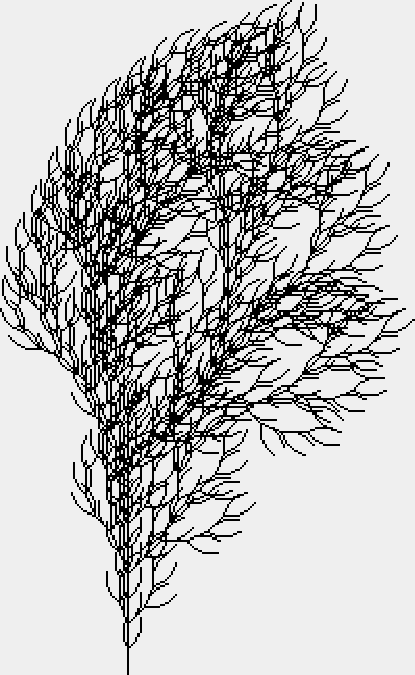
\includegraphics{arbres3}
\end{chapterfigure}

\forreviewers{I would like to present 3D like trees, however this implies to 
introduce so called generic L-Systems, which requires an
interpretation mechanism (parameters and expressions should be
evaluated) instead of a simple string replacement. Moreover the turtle
should be able to evolve in a 3d space. I do not know if this is worth
the complexity. One the other side I could try to use the 3d engine of
Squeak, and show some problems and their solutions. I suspect that
such an extension would take another chapter. Do you think that this
is interesting?  Would you like to read that?\\ Stef}

In this chapter we show how L-Systems are used to model plants.  We
present how theorical biologists, like Lindenmayer, enhanced simple
L-Systems to describe branching. Then we extend the \ct{Turtle} class
to support the needed behavior by creating a new class of \ct{Turtle}.

\section{L-System with Branching}
To represent plants or trees it is necessary to be able to model
branches. To that purpose, theoritical biologists introduced in
L-System the notion of branching. The idea is that to produce a branch
the current state of the turtle should first be stored, then the
turtle draws the branch hence modifying its state, then the state
before branching is restored and another branch with the same approach
can be drawn. Note that as branch can contains other branches, we have
to be able to store a collection of turtle states and restore then in
opposite order they have been stored: we need to store them into a
\emph{stack}.

To introduce such an idea into an L-System, the biologists introduced
the notion of storing the state of a turtle and restoring it.  Two new
symbols are added:

\begin{description}
\item{\ct{[}} pushes the current turtle state into the stack of turtle state.
\item{\ct{]}} pop the last stored state of the the stack and change the current turtle state accordingly. 
\end{description}

Here is the definition of the L-System that is shown in
Figure~\ref{fig:arbres1}.

\begin{tabbing}
\=aaa\=aaa\=aaa\=aaaaaaaaa\=aaaaaaaaa\=aaaaaaaaa\=aaaaaaaaa\=aaaaaaaaa\=aaaaaaaaa\kill
Plant 1. (Figure~\ref{fig:arbres1})\\
\>\>\>\> \emph{Axiom} \>\>F\\
\>\>\>\> \emph{Angle} \>\>25.7 degree\\
\>\>\>\> \emph{Rule}  \>\>F $\rightarrow$ F[+F]F[-F]F
\end{tabbing}

\begin{figure}
\centerline{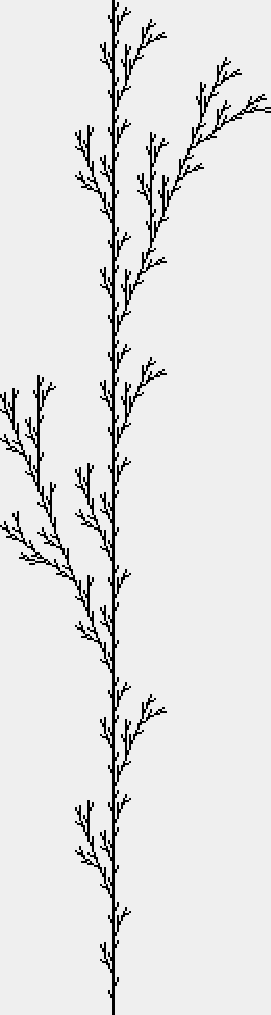
\includegraphics[height=9cm]{arbres1}}
\caption{Plant1. n = 5, 25.7 degree, F, F $\rightarrow$ F[+F]F[-F]F}
\label{fig:arbres1}
\end{figure}

From the implementation point of view, this L-System is created and
drawn as follow:

\begin{scriptwithtitle}{Using branching in a L-System}
| lsys |
lsys := self new.
lsys axiom: 'F'.
lsys add: (LSRule leftPart: 'F' rightPart: 'F[+F]F[-F]F').
lsys drawAtLevel: 4 length: 6 angle: 22.5
\end{scriptwithtitle}


\subsection{Some examples}
Here we propose you some L-Systems defining plants. 

\begin{figure}
\centerline{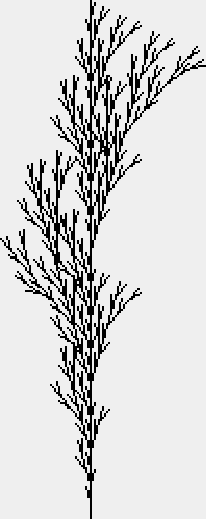
\includegraphics{arbres2}}
\caption{Plant 2. n = 5, 20 degree, F\newline F $\rightarrow$ F[+F]F[-F][F]}
\label{fig:arbres2}
\end{figure}


\begin{tabbing}
\=aaa\=aaa\=aaa\=aaaaaaaaa\=aaaaaaaaa\=aaaaaaaaa\=aaaaaaaaa\=aaaaaaaaa\=aaaaaaaaa\kill
Plant 2. (Figure~\ref{fig:arbres2})\\ 
\>\>\>\> \emph{Axiom} \>\>F\\
\>\>\>\> \emph{Angle} \>\>20 degree\\
\>\>\>\> \emph{Rule}  \>\>F $\rightarrow$ F[+F]F[-F][F]
\end{tabbing}


The following L-System produces the first picture of this chapter
after 4 iterations.
\begin{tabbing}
\=aaa\=aaa\=aaa\=aaaaaaaaa\=aaaaaaaaa\=aaaaaaaaa\=aaaaaaaaa\=aaaaaaaaa\=aaaaaaaaa\kill
Plant 3. (Chapter Picture)\\
\>\>\>\> \emph{Axiom} \>\>F\\
\>\>\>\> \emph{Angle} \>\>22.5 degree\\
\>\>\>\> \emph{Rule}  \>\>F $\rightarrow$ FF-[-F+F+F]+[+F-F-F]
\end{tabbing}


In the following L-Systems, the second rule is there to control the
length of the branches. This is a bit limited because the length can
only be a integer multiple of the distance the turtle moves forward.


\begin{tabbing}
\=aaa\=aaa\=aaa\=aaaaaaaaa\=aaaaaaaaa\=aaaaaaaaa\=aaaaaaaaa\=aaaaaaaaa\=aaaaaaaaa\kill
Plant 4.\\
\>\>\>\> \emph{Axiom} \>\>X\\
\>\>\>\> \emph{Angle} \>\>20 degree\\
\>\>\>\> \emph{Rule}  \>\>X $\rightarrow$ F[+X]F[-X]+X\\
\>\>\>\> \emph{Rule}  \>\>F $\rightarrow$ FF
\end{tabbing}



\begin{tabbing}
\=aaa\=aaa\=aaa\=aaaaaaaaa\=aaaaaaaaa\=aaaaaaaaa\=aaaaaaaaa\=aaaaaaaaa\=aaaaaaaaa\kill
Plant 5.\\
\>\>\>\> \emph{Axiom} \>\>X\\
\>\>\>\> \emph{Angle} \>\>25.7 degree\\
\>\>\>\> \emph{Rule}  \>\>X $\rightarrow$ F[+X][-X]FX\\
\>\>\>\> \emph{Rule}  \>\>F $\rightarrow$ FF
\end{tabbing}

\begin{tabbing}
\=aaa\=aaa\=aaa\=aaaaaaaaa\=aaaaaaaaa\=aaaaaaaaa\=aaaaaaaaa\=aaaaaaaaa\=aaaaaaaaa\kill
Plant 6. (Figure~\ref{fig:arbres6})\\
\>\>\>\> \emph{Axiom} \>\>X\\
\>\>\>\> \emph{Angle} \>\>22.5 degree\\
\>\>\>\> \emph{Rule}  \>\>X $\rightarrow$ F-[[X]+X]+F[+FX]-X\\
\>\>\>\> \emph{Rule}  \>\>F $\rightarrow$ FF
\end{tabbing}

\begin{figure}
\centerline{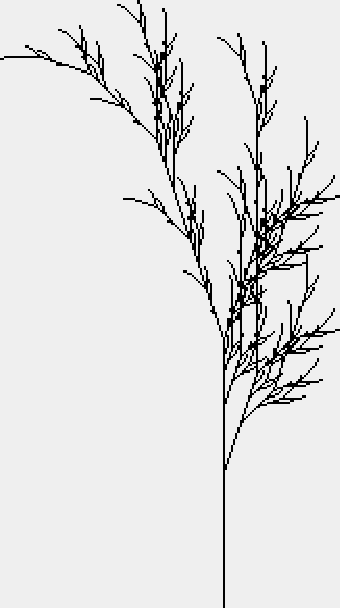
\includegraphics{arbres6}}
\caption{n = 5, 22.5 degree, X, F $\rightarrow$  FF, X $\rightarrow$ F-[[X]+X]+F[+FX]-X}\label{fig:arbres6}
\end{figure}

\section{A Turtle with Memory}
To implement the semantics of \[ and \], i. e., to store or restore
the state of a turtle, we have to implement some new behavior. This
behavior, maintaining a collection of turtle states, storing or
restoring them is definitively a new responsibility that has to do
with turtle behavior, so we will add this new behavior to the class
\ct{Turtle}.  In fact, we prefer to extend the class \ct{Turtle} by creating 
a subclass of \ct{Turtle} because not all the turtles have to have
this specific behavior. Figure~\ref{fig:turtleMemory} presents the
solution we propose you.


\begin{figure}[!htbp]
\centerline{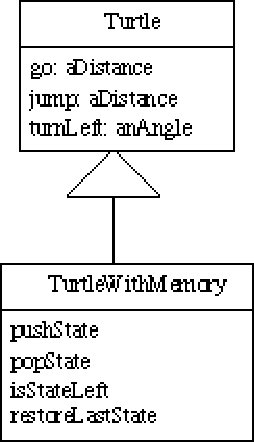
\includegraphics{turtleMemory}}
\caption{Extending the \ct{Turtle} class by creating a subclass: \ct{TurtleMemory}.}
\label{fig:turtleMemory}
\end{figure}


\subsection{The strategy} 

There are different ways to implement the new behavior that we
need. However, the simplest one is to see that the states that we want
to store or restore behave like a \emph{stack} of plates. Stacks are
one of the elementary data-structures like collection, hash-table, or
queues that any programmer has to master.  Let's illustrate how a
stack works: if we store S1, S2 and S3 three states on a stack in the
chronological order, then the top of the stack is S3 and the bottom
S1. Stacks are \emph{last in first out structure}: S1 will be the
lastest state to be popped out the stack. This is exactly what we
want: we want to store the state of a turtle before drawing a branch
(which may contain other branches) and come back to this state later.
Popping a stack means that the top of the stack is removed and that
the element below becomes the top of the stack. Pushing an element
into the stack means that the element becomes the top of the stack.


\begin{scriptwithtitle}{Behavior of a stack}
stack push: s1.
stack push: s2.
stack push: s3.
stack pop. \emph{returns s3}
stack push: s4.
stack pop. \emph{returns s4}
stack pop. \emph{returns s2}
\end{scriptwithtitle}

\forreviewers{Here an illustration is missing}


\subsection{Implementing a stack} 

If you look in Squeak using a class browser for a class whose name
contains \ct{Stack} or using a method finder, you will not find a
class directly implementing a stack of objects. Now if you analyze a
bit a stack you can see that: (1) a stack is a kind of ordered
collection. Its elements are ordered based on the order in which they
are pushed on the stack and (2) we are able to add or remove
dynamically elements. These two observations make the instances of
\ct{OrderedCollection} good candidates for representing a stack. Now
we have to see how pushing an element and popping the stack can be
implemented. Let'us take the following convention: the top of the
stack is the last element of the collection.

\paragraph{Do it.} Look at the methods defined on the class \ct{OrderedCollection}
and find two methods that can be used to implement the following methods:

\begin{itemize}
\item one, named \ct{push:}, that could
be used to implement the addition of an element on the top of the
stack. According to the convention we chose, the element should be
added at the end of the collection. Note that as ordered collections
grow dynamically we do not have to check if we overpass the size of
the collection.

\item another method, named \ct{pop}, that could be
used to implement the action to pop the stack, i.e., returns the top
element and remove it from the stack.
\end{itemize}

\subsection{Subclassing the class \ct{Turtle}}
The state of a turtle that we need to store and restore is not
represented by a single object but composed by two objects: a point
representing its position and a number representing its direction. So
we have several possibilities to represent a stack of turtle state: we
can have one stack for the position and one stack for the direction
and manipulate them in synch, or bundling together the position and
direction using a pair of objects and using one single stack. We chose
the second approach.

\paragraph{About \ct{Association}.} To create a pair\index{pair}\index{association}
of objects, we create an instance of the class \ct{Association} by
sending to any object the message \ct{->} \index{association creation}
with as argument the other object we want to associate with. Then
accessing the elements of the association is performed by sending the
messages \ct{key} or \ct{value} to the association. The
\scriptref{scr:association} illustrates the creation and access to an
association. For more information browse the class \ct{Association}.

\begin{scriptwithtitle}{Example of association use}\label{scr:association}
| anAssociation |
anAssociation := \#caro -> 3.
anAssociation key \emph{returns \#caro}
anAssociation value \emph{returns 3}
\end{scriptwithtitle}


\paragraph{Class Definition.}
Define a class named \ct{TurtleWithMemory} subclass of the class
\ct{Turtle}. This class has an intance variables named \ct{stateStack}
that represents a stack of turtle state.

\hidden{
\begin{method}
Turtle subclass: #TurtleWithMemory
   instanceVariableNames: 'stateStack'
   classVariableNames: ''
   poolDictionaries: ''
   category: ''
\end{method}}

\forreviewers{This part will certainly migrate to a chapter going deeper into this topic}
\subsection{Instance Variable Initialization} \label{sec:variableinitialization}
In Smalltalk, instance 
variables are initialized with the \ct{nil} object, instance of the
class \ct{UndefinedObject} --- this means that they value is the
object \ct{nil}. That's why before using an instance variable, we have
to initialize it with a value consistent with its future use. There is
no predefined way in Smalltalk to initialize instance variables.  One
way is to invoke a method often named by convention
\ct{initialize} that sets the value of the instance variables as soon
as the instance is created.  However, what is important is that such
an initializing method should be \emph{systematically} invoked on the
newly created object, else we could forget to invoke it and obtain an
object in an inconsistent state.

To ensure that an initializing method is automatically invoked, we can
specialize the class method \ct{new}, whose responsibilities is to
create new instances of the class to which new is sent. There are two
key points not to forgot: (1) the creation of instance should be
invoked, and (2) the newly created instance should returned.  A method
\ct{new} defined on an hypothical class \ct{XXX} would look as the following:

\begin{method}
XXX class>>new
 
    |inst|
    inst := super new.
    inst initialize.
    ^ inst
\end{method}

First, the new instance is created by invoking the method \ct{new},
then an initializing method, called \ct{initialize} is invoked on this
newly created instance and finally the instance is returned. Note that this 
method is equivqlent to the following one: 

\begin{method}
XXX class>>new

	^ super new initialize
\end{method}

The method \ct{initialize} can initialize the value of some instance
variables of the instance as follow two forms are possible using
direct access to instance variables or using accessors if they have
been defined:

\begin{method}
XXX>>initialize
 
    myInst1 := 0
\end{method}

\begin{method}
XXX>>initialize
 
    self myInst: 0
\end{method}

\forreviewers{Until there the part will be moved in another place}


\paragraph{Initializing turtle with memory.}
Before reproducing the initialization schema, we should look at the
superclasses of the class \ct{TurtleWithMemory} to check if they do
not already redefine the method \ct{new}.  In such a case there is no
need to redefine it again and we just need to redefine the
\ct{initialize} method. As you can find, the superclass \ct{Morph}
redefine the method \ct{new} as follow, so there is no need to
redefine it.

\begin{method}
Morph class>>new

	^ super new initialize
\end{method}

Define the method \ct{initialize} to set the value of  the instance variable
\ct{stateStack} to an empty ordered collection as follow.

\begin{method}
TurtleWithMemory>>initialize
   "initialize the state stack"
   
   super initialize.
   stateStack := OrderedCollection new.
\end{method}

As a TurtleWithMemory instance has all the behavior that a normal
turtle has \emph{plus} the extra behavior necessary to store and
restore turtle's state, we have to invoke the \ct{initialize} method
defined in the superclass of \ct{TurtleWithMemory}, i.e.,
\ct{Turtle} or its superclass. This is the purpose of the expression \ct{super
initialize}.  Then the instance variable specific to the class
TurtleWithMemory is initialized to hold an empty collection, instance
of \ct{OrderedCollection} that represents the turtle state stack.


\paragraph{Push/Pop.}
Using the knowledge you gain about stack implementation, define the
following methods:
\begin{itemize}
\item \ct{pushState} adds to the stack of turtle states the current state of
 the turtle. 
\item \ct{popState} returns the top element of the stack and make the
 subsequent element the new top. Do not check if the stack is empty. 
\item \ct{isStateLeft} checks whether the stack is empty.
\item \ct{restoreLastState} changes the current turtle state to be the last ones that have been stored in the state stack.
\end{itemize}

\paragraph{Extending the L-System Interpretation.}
Now you just have to extend the method \ct{interpretSymbol: aChar
length: len angle: degree} to take into account the interpretation of
symbols: [ and ]. Think about reusing the method
\ct{interpretSymbol:length:angle:} defined on the class
\ct{Turtle}.

\begin{exonofig} Chose as convention that the beginning of the collection is
the top of the stack and reimplement the functionality. Note however
that the implementation of ordered collection makes more efficient the
first solution.
\end{exonofig}

\begin{exonofig}Chose to represent the turtle state stack as two stacks: one stack for the position and one for the direction.
\end{exonofig}


\section{Stochastic L-Systems}
Up until now a given L-System produces always the same plant in a
deterministic manner. There is no random decision. To introduce more
realistic and different plants, biologists introduce in L-System the
notion of random selection of a rule, hence the term \emph{stochastic}
L-Systems. The idea is simple, every rule is given a probability to be
selected and while checking if a rule is applicable the L-System
selected them according to this probability.

\begin{tabbing}
\=aaa\=aaa\=aaa\=aaaaaaaaa\=aaaaaaaaa\=aaaaaaaaa\=aaaaaaaaa\=aaaaaaaaa\=aaaaaaaaa\kill
\>\>\>\> \emph{Axiom} \>\>F\\
\>\>\>\> \emph{Angle} \>\>25.7 degree\\
\>\>\>\> \emph{Rule}  \>\>F .33 $\rightarrow$ F[+F]F[-F]F\\
\>\>\>\> \emph{Rule}  \>\>F .33 $\rightarrow$ F[+F]F\\
\>\>\>\> \emph{Rule}  \>\>F .34 $\rightarrow$ F[-F]F
\end{tabbing}


We will not propose any solution and let you think about the solution. 
However to help a bit here are some points that you should think of: 
\begin{itemize}
\item Do the rule have equal probability? This can have an impact on when to assign a rule 
its probability. Once the rule is created or once all the rules have
been added. The simplest solution being to assign individual
probability to each rule and let this responsibility to the
programmer. A next step is then to let the system computes the
probability to the rules.

\item Is a probability assign to a rule? Presumbly yes, the probability can be just an 
extra property of a rule. Take care to initialize it to a valid value. 
\end{itemize}

The following expression shows how a random number between 0 and 10
excluded can be generated.
\begin{scriptwithtitle}{Random Number}
10 atRandom
\end{scriptwithtitle}


\ifx\wholebook\relax\else\end{document}\fi
